\documentclass[10pt,a4paper]{article}
\usepackage[utf8]{inputenc}
\usepackage{amsmath,amsfonts,amssymb,float,wrapfig,titling,latexsym}
\usepackage[left=2.5cm,right=2.5cm,top=2.5cm,bottom=2.5cm]{geometry}
\usepackage[usenames, dvipsnames]{color}

\usepackage{graphicx}
\graphicspath{{images/}}

\usepackage{hyperref}
\hypersetup{colorlinks=true, linkcolor=blue, urlcolor=red}
\usepackage[backend=biber, style=numeric, sorting=none]{biblatex}
\addbibresource{refs.bib}

\usepackage[labelformat=simple]{subcaption}
\renewcommand\thesubfigure{(\alph{subfigure})}


\def\session{\ifcase\month\or
	January\or February\or March\or April\or May\or June\or
	July\or August\or September\or October\or November\or December\fi
	,\space \number\year}

\title{
\includegraphics[height=4cm, scale=1]{iitbbs.png}\\
	\LARGE \bf  Droplet generation from cone jet using electrostatic forces: A hybrid lattice Boltzmann-finite difference based numerical study}
\author{
	\LARGE Himadri Sekhar Basu\\
	\LARGE S18ME09004\\[4ex]
	\Large \bf Under the guidance of\\
	\Large Dr. Sasidhar Kondaraju\\[6ex]
	\LARGE \bf School of Mechanical Sciences\\
	\LARGE \bf Indian Institute of Technology, Bhubaneswar\\[6ex]}
\date{\LARGE \today}

\begin{document}

\pagenumbering{gobble}
\maketitle
\clearpage

\pagenumbering{roman}
\tableofcontents
\clearpage
\listoffigures
\clearpage
\listoftables
\clearpage

\pagenumbering{arabic}
\section{Introduction}
Using EKI we can generate droplet\cite{Bahga-2010}
\begin{figure}[h!]
	\centering
	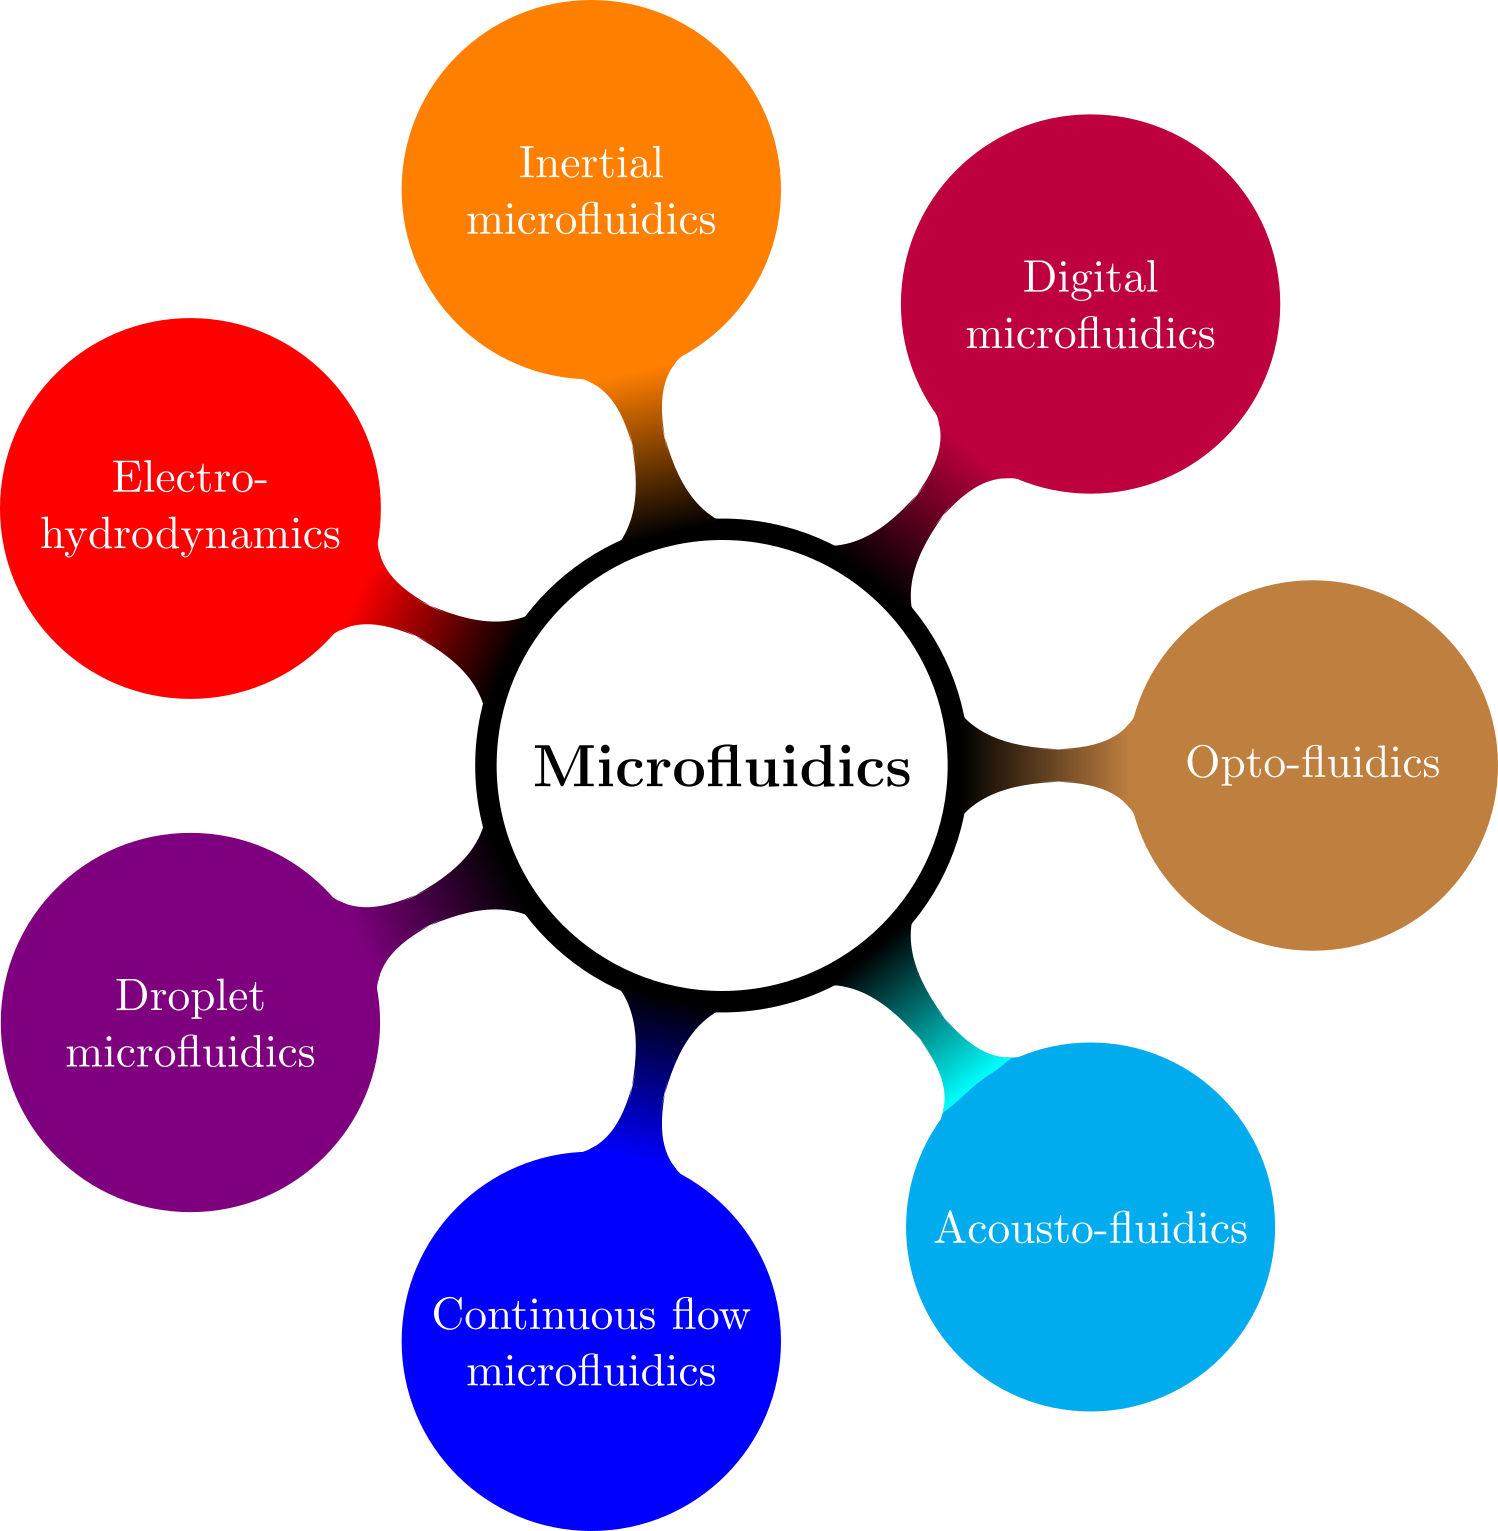
\includegraphics[width=0.5\linewidth,scale=1]{microfluidic_sub_fields}
	\caption{Various sub-fields of Microfluidics.}
	\label{fig:microfluidicsubfields}
\end{figure}

\subsection{Objective}
\subsection{Motivations}
( Benefits- economical)
\subsection{Financial}
(Can be in terms of efficiency although currency numbers are more preferred).
\subsection{Work impact}
Brief explanation of work impact ( Broad area)
\clearpage

\section{Project substance}
This should include 2 small paragraphs of brief methodology i.e., what is my interest, what I am trying to achieve through my experimental setup/numerical scheme.
\clearpage

\section{Contents of research}
\subsection{Previous studies}
\subsection{Limitations}
\subsection{Experience to achieve results}
(You have studied literature and now procuring a experimental setup, with this you have to convince the readers that you are capable of achieving results. It should be valid).
\subsection{Details about research}
(All the study parameters which I will be studying and varying)
\subsection{Challenges}
(Which I will be facing while doing my experimental project)
\clearpage
\section{Methodology}
(Detailed experimental and analytical process to be adopted or a flowchart to defend same including brief explanations).\\
Mention the parameters selected for study, how you are going to change them and why?...for each objective and also show analysis.
\section{Work plan}
Make it in two parts. One is timeline where your plan is divided in terms of months and second is here your plan is divided in terms of years.
\section{Anticipate results and potential contribution}
This should include both short term and long term results. Also there should be a link directing impact of short term results on long term results like impact on society or monetary gains for some section of people or some countries.

\printbibliography[heading=bibintoc]
\end{document}